\newcolumntype{P}[1]{>{\centering\arraybackslash}p{#1}}
\newcolumntype{M}[1]{>{\centering\arraybackslash}m{#1}}
\section{Divide and Conquer II}
\begin{itemize}
	\item Last time, we saw Karatsuba's \( O(n^{1.6}) \) multiplication algorithm, and did a formal recap on 
		\( O(\cdot) \) and \( \Omega(\cdot) \) notation. We ended with recurrence relations and the master theorem. 
	\item Remember that \( a \) is the number of subproblems we have, \( b \) is the factor by which the problem size 
		shrinks, and \( n^{d} \) is the amount of computation per node. Note that if the work at every layer 
		we have \( c \cdot n^{d} \) work instead, then the runtimes are instead described by \( \Theta \) relationships.  
	\item One way to interpret the comparison between \( a \) and \( b^{d} \) is that when \( a > b^{d} \), the tree 
		is very large -- there are a lot of subproblems. This means that most of the work is at the bottom of the tree, 
		so we have an \( O(n^{\log_ba}) \) runtime. 

		Conversely, when \( a < b^{d} \), then the tree is very narrow, this means that most of the work is at the top of the tree
		(or alternatively, the work is concentrated in the combination step), which is why we have an \( O(n^{d}) \) runtime. 
		
		When the branches perfectly equals the amount of work per layer, then we get an \( O(n^{d}\log n) \) runtime.
\end{itemize}
\subsection{Matrix Multiplication}
\begin{itemize}
	\item We've shown that integer multiplication can be optimized, but what about matrix multiplication? As a reminder, 
		the product of two \( n \times n \) matrices \( X, Y \) is an \( n \times n  \) matrix  \( Z \), where every 
		entry \( z_{ij} \) is the dot product of row \( i \) in \( X \) with column \( j \) in \( Y \). 
	\item What's the runtime of this multiplication? In this case, we want a runtime in relation to the number of rows and 
		columns. For simplicity, we will deal with square matrices, so we only care about an \( n \). We'll also assume 
		that integers have a small number of bits, so they can be multiplied in constant time. 
	\item To answer this, we first ask: what is the runtime of computing the dot-product of two vectors of size \( n \)? Well, 
		there are \( n \) multiplications, so the dot product is \( O(n) \). Then, since there are \( n^2 \) dot products (one 
		per cell in the \( n \times n \) matrix, then the total runtime will be \( o(n \cdot n^2) = O(n^3) \). 
	\item Let's try breaking up matrices into smaller matrices, of size \( \frac{n}{2} \times \frac{n}{2} \):
		\begin{center}
			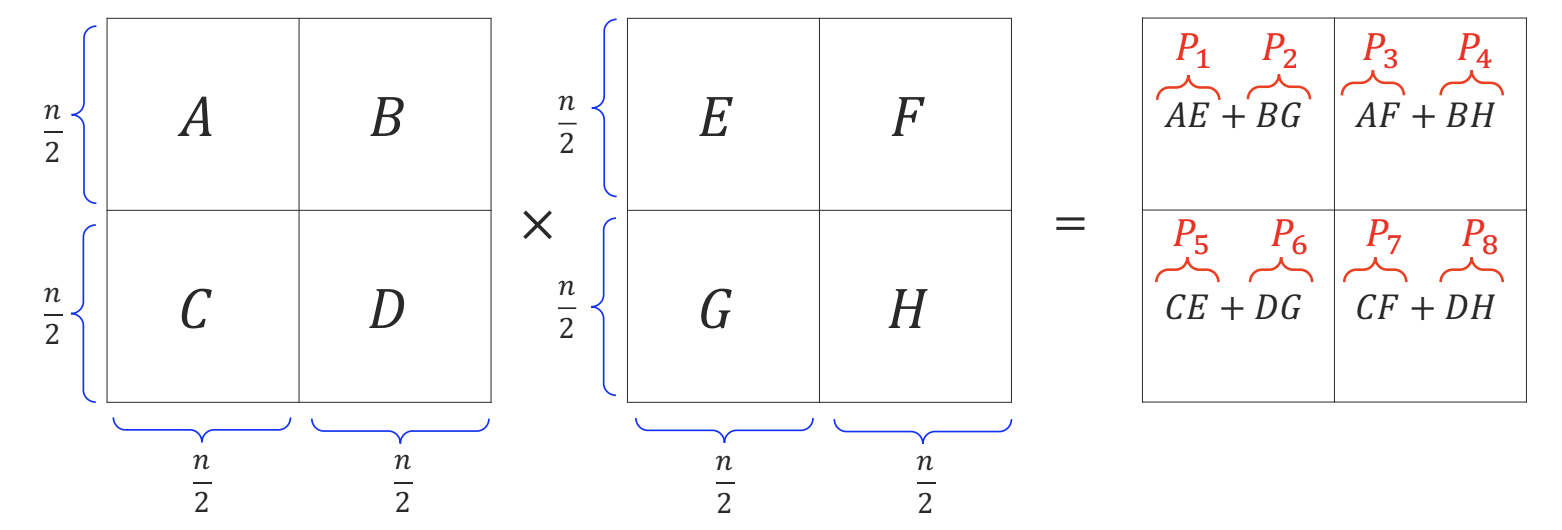
\includegraphics[scale=0.6]{matrix-multiplication.png}
		\end{center}
		At each layer we generate \( 8 \) problems, of size \( \frac{n}{2} \). At every step, we have work that's on the order 
		of \( O(n^2) \); this includes breaking up the problem, adding the matrices, and appending matrices to one another. This 
		gives a recurrence relation: 
		\[
		T(n) = 8T\left( \frac{n}{2} \right) + O(n^2)
		\] 
		Using the master theorem, this still gives us \( O(n^3) \) runtime! How do we make this better? We take inspiration from 
		Karatsuba's algorithm, and notice that the way we optimized that was by reducing the number of subproblems. If we can 
		get away with generating less than 8 subproblems, then we will get a speedup.  
\end{itemize}
\subsection{Strassen's Algorithm}
\begin{itemize}
	\item The approach is very similar to Karatsuba's, but this time for matrices. He went from 8 subproblems down to 7. He 
		essentially creates the following problems:
		\begin{align*}
			Q_1 &= A(F - H) \\
			Q_2&= (A + B)H \\
			Q_3&= (C + D)E \\
			q_4 &=  D(G - E) \\
			Q_5 &=  (A + D)(E + H) \\
			Q_6 &= (B - D)(G + H) \\
			Q_7 &=  (A - C)(E + F) \\
		\end{align*}
		and combined them in the following way:
		\renewcommand{\arraystretch}{4}
		\begin{center}
			\begin{tabular}{|M{2.5cm}|M{2.5cm}|}
				\hline
				\( Q_5 + Q_4 - Q_2 + Q_6 \) & \( Q_1 + Q_2 \) \\ \hline 
				\( Q_3 + Q_4 \) & \( Q_1 + Q_5 - Q_3 - Q_7 \)\\ \hline
			\end{tabular}
		\end{center}
		Yeah, it looks insane and is insane, but it works.
		%figure out how to center these matrices 
		\renewcommand{\arraystretch}{1}
	\item So now, our recurrence relation is:
		\[
		T(n) = 7T\left( \frac{n}{2} \right) + O(n^2)
		\] 
		which from the Master Theorem, this has runtime \( O(n^{\log_2 7}) \approx O(n ^{2.8}) \). Recent advancements have 
		brought this exponent down to \( O(n^{2.34}) \) approximately.
\end{itemize}
\subsection{Median Selection}
\begin{itemize}
	\item Given an array \( S \) of \( n \) numbers and \( k \in \{1, 2, \dots, n\}  \), the \( k \)-select problem (written 
		as \( \text{SELECT}(S, k) \)) asks us 
		to find the \( k \)-th smallest element within \( S \). \( k = 1 \) selects the minimum, \( k = n \) selects
		 the maximum, and \( k = \left\lceil n / 2 \right\rceil  \) selects the median. 
	 \item A brute-force algorithm that runs in \( O(n \log n) \) is to just sort the array, then output the \( k \)-th element. 
		 Can we do better? Specifically, can we do \( O(n) \)?
	 \item For \( \text{SELECT}(S, 1) \) an \( O(n) \) algorithm would be to just keep track of the minimum element. If we were 
		 interested in \( \text{SELECT}(S, 2) \), then we could run \textsc{select(S, 1)} twice -- on the first ieration, 
		 remove the minimum element, then running \( \text{SELECt}(S, 1) \) again returns the second smallest 
		 element. 
	 \item Does this produce an \( O(n) \) algorithm for \( \text{SELECT}(S, n / 2 \)? No, because this would mean that we 
		 would be running  \( \text{SELECT}(S, 1) \)  \( n / 2 \) times, and if each is \( O(n) \) then we get 
		 an overall runtime of \( O(n^2) \). 
	 \item Let's take the Divide and Comquer approach: imagine we're given a pivot \( v \) (like in quicksort), and split the array 
		 into three pieces:
		 \begin{itemize}
		 	\item \( S_L \) : elements in \( S \) that are less than \( v \) 
			\item \( S_v \) : elements in \( S \) that are equal to \( v \) 
			\item \( S_R \) : elements in \( S \) that are larger than \( v \)
		 \end{itemize}
		Splitting elements in  \( S \) into these two portions takes \( O(n) \) time, since we can just run through the array 
		and place elements accordingly. Effectively, this sorts our array into chunks, which allows us to recurse on smaller 
		subproblems. 
	\item Now suppose we want to compute \( \text{SELECT}(S, k) \):
		\begin{itemize}
			\item If \( k \le \text{len}(S_L) \), then the \( k \)-th smallest elemet lives in \( S_L \), so we run 
				\( \text{SELECT}(S_L, k) \).
			\item If \( \text{len}(S_L) < k \le \text{len}(S_L) + \text{len}(S_v)\), then the \( k \)-th smallest element is exactly 
				the value of the pivot since \( k \) doesn't go past \( S_L \) and \( S_v \) combined, so we return \( v \). 
			\item If \( \text{len}(S_L) + \text{len}(S_v) < k \), then we recurse on \( S_R \), but we have to be careful 
				since the \( k \)-th smallest element would be the \( k - \len(S_L) - \text{len}(S_v) \) in \( S_R \). So, 
				we return \( \text{SELECT}(S_R, k - \len(S_L) - \len(S_v) \)
		\end{itemize}
	\item In summary, our recurrence relation is given by:
		\[
		T(n) = \begin{cases}
			T(\len(S_L)) + O(n) & k \le \len(S_L)\\
			T(\len(S_R)) + O(n) & \len(S_L) + \len(S_v) < k\\
			O(n) & \len(S_L) < k \le \len(S_L) + \len(S_v)
		\end{cases}
		\] 
		Note that the lengths of \( S_L \) and \( S_R \) depend on the choice of the pivot, so how do we select a good pivot? 
	\item Ideally, we'd want a pivot such that \( \max(\len(S_L), \len(S_R)) \) to be relatively small. This means that 
		we effectively want to pick a pivot that's as close to the median as possible.  
	\item Given an ideal pivot, where we select the median, then we know that \( \len(S_L) \le  n / 2 \) and 
		\( \len(S_R) \le  n / 2 \). Therefore, we only recurse on half the array every single time, so our recurrence 
		relation is:
		\[
		T(n) \le  T\left( \frac{n}{2} \right) + O(n)
		\] 
		By the master theorem, this would take \( O(n) \) runtime. So in the best case scenario, this way of computing the median 
		does take \( O(n) \) time!
	\item We can't \textit{always} pick the median (obviously), so let's relax our constraints a little and consider a pivot 
		to be "good" when it's between the \( \frac{n}{4} \)-th smallest and \( \frac{3n}{4} \)-th smallest element. This 
		makes the maximum length of \( S_L \) and \( S_r \) to be at most \( \frac{3n}{4} \). This is because
		there are at least \( \frac{n}{4} \) elements that are never looked at again if the pivot is good. The recurrence 
		relation for this would be:
		\[
		T(n) \le  T\left( \frac{3n}{4} \right)  + O(n)
		\] 
		which by the master theorem, would still be \( O(n) \).  
	\item So how do we pick a good pivot? We could just choose one uniformly at random from \( S \), and we'll show later that 
		this gives an \( O(n) \) algorithm in expectation. The other alternative is to find a good pivot deterministically, but 
		this is much harder and in practice it's slower than using a random pivot. 
	\item Now let's prove the \( O(n) \) expected runtime. 
		
		In our case, 
		we know that a good pivot is chosen when our problem size drops to \( 3 /4 \) or less than the previous array size, 
		so we can partition the tree layers into phases where this happens. 

		Because a new phase begins when the array size shrinks by \( \frac{3}{4} \), then we know that at phase \( i \), 
		the problem size is at most \( (3 / 4)^{i} \cdot n \), with equality if we've picked only good pivots up until this point.
		Let \( X_i \) be the random variable that denotes the length of phase \( i \). Per node, we compute 
		\( c \cdot n \) operations, so the contribution at any phase \( i \) is given by 
		\( X_i \cdot c\left( \frac{3}{4} \right) ^{i} \cdot n \). Therefore, now we have:
		\[
			T(n) \le  \sum_{i = 0}^{\log_{4 / 3}(n)}X_i \cdot c\left( \frac{3}{4} \right) ^{i}n
		\] 
		\comment{Note that the problem size is \( \left( \frac{3}{4} \right)^{i}n \).}

		Then, in expectation, we're looking for:
		\[
			E[T(n)] \le  \sum_{i = 0}^{\log_{4 / 3}(n)}E[X_i] \cdot c \left( \frac{3}{4} \right) ^{i}n
		\] 
		So we want to find \( E[X_i] \). Recall that \( X_i \) is directly a function of the number of times a bad pivot 
		was chosen, which happens \( 50\% \) of the time. This means that in expectation, the length of \( X_i \) is 2, 
		since we expect that a good pivot is chosen \( 50\% \) of the time (and thus we enter \( X_{i+1} \) ). So in expectation, 
		we have:=
		\[
			E[T(n)] \le \sum_{i = 0}^{\log_{4 / 3}(n)} 2 c\left( \frac{3}{4} \right) ^{i} n
		\] 
		which you can check using the tree method, does give \( O(n) \). 
\end{itemize}
